\begin{enunciado}{\ejercicio}
  Probar que para todo $n \geq 3$ vale que
  \begin{enumerate}[label=\roman*)]
    \item la cantidad de diagonales de un polígono de $n$ lados es
          $\frac{n(n-3)}{2}$.
    \item la suma de los ángulos interiores de un polígono de $n$ lados es
          $\pi(n-2)$.
  \end{enumerate}
\end{enunciado}

\begin{enumerate}[label=\roman*)]
  \item La cantidad de diagonales de un polígono de $n$ lados es $\frac{n(n-3)}{2}$.\par
        Ejercicio donde hay que encontrar una fórmula a partir de algún método \textit{creativo} para luego probar por inducción.\par
        $$
          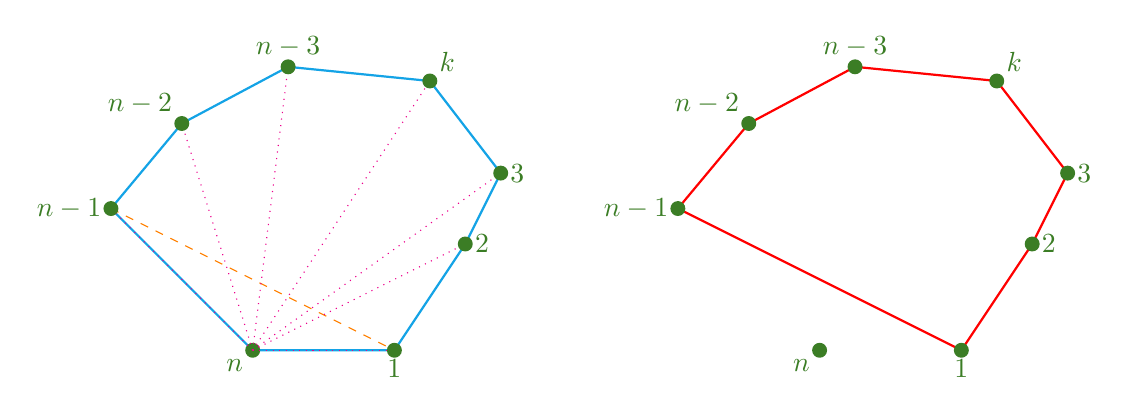
\begin{tikzpicture}[scale=0.9]
            \coordinate (n) at (0,0);
            \coordinate (1) at (2,0);
            \coordinate (2) at (3,1.5);
            \coordinate (3) at (3.5,2.5);
            \coordinate (k) at (2.5,3.8);
            \coordinate (n-3) at (0.5,4);
            \coordinate (n-2) at (-1,3.2);
            \coordinate (n-1) at (-2,2);

            \draw[dashed, orange] (n-1) -- (1);
            \draw[thick, Cerulean] (n) -- (1) -- (2) -- (3) -- (k) -- (n-3) -- (n-2) -- (n-1) -- cycle;

            \foreach \point/\position in {n/below left, 1/below, 2/right, 3/right, k/above right, n-3/above, n-2/above left, n-1/left}
              {
                \draw[dotted, magenta] (n) -- (\point);
                \fill[OliveGreen] (\point) circle (3pt) node [\position] {$\point$};
              }
            \begin{scope}[xshift=8cm]
              \coordinate (n) at (0,0);
              \coordinate (1) at (2,0);
              \coordinate (2) at (3,1.5);
              \coordinate (3) at (3.5,2.5);
              \coordinate (k) at (2.5,3.8);
              \coordinate (n-3) at (0.5,4);
              \coordinate (n-2) at (-1,3.2);
              \coordinate (n-1) at (-2,2);

              \draw[thick, red] (n-1) -- (1) -- (2) -- (3) -- (k) -- (n-3) -- (n-2) -- (n-1) -- cycle;

              \foreach \point/\position in {n/below left, 1/below, 2/right, 3/right, k/above right, n-3/above, n-2/above left, n-1/left}
                {
                  \fill[OliveGreen] (\point) circle (3pt) node [\position] {$\point$};
                }
            \end{scope}

          \end{tikzpicture}
        $$

        Se desprende del gráfico el siguiente razonamiento:

        En el polígono \blue{azul} de $n$ lados voy a tener una \textit{cantidad de
          diagonales} dada por la sucesión $d_n$. El polígono \red{rojo}, tiene un lado menos,
        por lo tanto la sucesión que describe su \textit{cantidad de diagonales} es $d_{n-1}$.

        Las líneas \magenta{punteadas} son las diagonales de $d_n$ que \ul{no} estarán en
        $d_{n-1}$.

        La idea es encontrar una relación entre ambas sucesiones. Al modificar el polígono sacando el vértice $n$ pierdo las
        \magenta{diagonales punteadas} desde el nodo $2$ hasta $n-2$ que
        serían $\magenta{n-3}$ en total y no hay que olvidarse también que pierdo la \orange{diagonal naranja} que conectan el vértice $1$ con el $n-1$:
        $$
          \blue{d_n} = \red{d_{n-1}} + \orange{1} +\magenta{n-3} = d_{n-1} + n - 2
          \sii \cajaResultado{d_n = d_{n-1} + n - 2}
        $$

        Ahora inducción:

        Quiero probar la siguiente proposición:
        $$
          p(n): d_n = \frac{n(n-3)}{2} \paratodo n \geq 3
        $$
        \textit{Caso Base: }
        $$
          p(\blue{3}) : \frac{\blue{3} (\blue{3} - 3)}{2} = 0,
        $$
        lo cual es verdad para el triángulo.

        \textit{Paso inductivo: }
        Asumo que
        $$
          p(\blue{k}) : \ub{d_{\blue{k}} = \frac{\blue{k} (\blue{k} - 3)}{2}}{\text{\purple{hipótesis inductiva}}}
        $$
        es verdadera para algún $k \en \naturales_{\geq 3}$.

        Entonces quiero probar que:
        $$
          p(\blue{k+1}): d_{\blue{k+1}} =
          \frac{(\blue{k+1})(\blue{k + 1} - 3)}{ 2 }
          =
          \frac{(k+1)(k - 2)}{2}
        $$
        también sea verdadera.

        Arranco por la proposición $p(\blue{k+1})$ y uso la \purple{hipótesis inductiva}:
        $$
          d_{k+1}
          \igual{def}
          d_k + k - 1
          \igual{\purple{HI}}
          \purple{\frac{k (k-3)}{2}} + k - 1 =
          \frac{k^2 - k - 2}{2} \igual{\red{!}}
          \frac{(k+1)(k-2)}{2}
        $$

        Como $p(3),\, p(k) \text{ y } p(k+1)$ resultaron verdaderas, por el principio de inducción $p(n)$ es verdadera $\paratodo n \en \naturales_{\geq 3}$

  \item la suma de los ángulos interiores de un polígono de $n$ lados es $\pi(n-2)$.
        $$
          \begin{tikzpicture}[scale=0.9]
            \coordinate (n) at (0,0);
            \coordinate (1) at (2,0);
            \coordinate (2) at (3.2,1.5);
            \coordinate (3) at (3.7,2.8);
            \coordinate (k) at (2.5,3.8);
            \coordinate (n-3) at (0.5,4);
            \coordinate (n-2) at (-1,3.2);
            \coordinate (n-1) at (-2,2);

            \draw[dashed, green] (n-1) -- (1);
            \draw[ultra thick, cyan] (n) -- (1) -- (2) -- (3) -- (k) -- (n-3) -- (n-2) -- (n-1) -- cycle;

            \draw[dashed, green] (n-1) -- (1);
            \draw[ultra thick, cyan] (n) -- (1) -- (2) -- (3) -- (k) -- (n-3) -- (n-2) -- (n-1) -- cycle;

            \pic [draw, angle eccentricity=1.5] {angle = 1--n--n-1};
            \pic [draw, angle eccentricity=1.5] {angle = 2--1--n};
            \pic [draw, angle eccentricity=1.5] {angle = 3--2--1};
            \pic [draw, angle eccentricity=1.5] {angle = k--3--2};
            \pic [draw, angle eccentricity=1.5] {angle = n-3--k--3};
            \pic [draw, angle eccentricity=1.5] {angle = n-2--n-3--k};
            \pic [draw, angle eccentricity=1.5] {angle = n-1--n-2--n-3};
            \pic [draw, angle eccentricity=1.5] {angle = n--n-1--n-2};

            \pic [draw, red, angle eccentricity=1.5, angle radius=1cm] {angle = n-1--1--n};
            \pic [draw, red, angle eccentricity=1.5, angle radius=0.7cm] {angle = 1--n--n-1};
            \pic [draw, red, angle eccentricity=1.5, angle radius=1cm] {angle = n--n-1--1};

            \foreach \point/\position in {n/below left, 1/below, 2/right, 3/right, k/above right, n-3/above, n-2/above left, n-1/left}
              {
                \fill[OliveGreen] (\point) circle (3pt) node [\position] {$\point$};
              }
          \end{tikzpicture}
        $$
        En este caso estoy generando la suma de los ángulos internos de 2 polígonos,
        uno con $\alpha_n$ de $n$ lados y otro con $n-1, \alpha_{n-1}$.

        Es más claro en este caso que al sacarle un lado, estoy formando un triángulo
        {\tiny(en el gráfico con vértices $n$, $n-1$, 1)}
        que tiene como suma de sus ángulos internos $\pi$, entonces afirmo
        $\alpha_{n+1} \igual{$\llamada1$} \alpha_n + \pi $.

        Ahora pruebo por inducción lo pedido:
        $$
          p(n): \alpha_n = \pi(n-2) \paratodo n \geq 3
        $$

        Arrancamos inducción:

        \textit{Caso Base: }
        $$
          p(3): \pi(3-2) = \pi,
        $$
        lo cual es verdad para el triángulo, como aprendiste en el secundario.

        \textit{Paso inductivo }, asumo que:
        $$
          p(k): \ub{\alpha_k = \pi(k-2)}{\text{\purple{hipótesis inductiva}}}
        $$
        es verdadero para algún $k \en \naturales_{\geq 3}$, entonces también quiero que:
        $$
          p(\blue{k+1}): \alpha_{\blue{k+1}} = \pi(k-1)
        $$
        también sea verdadero.

        Arranco con la definición y uso la hipótesis inductiva:
        $$
          \alpha_k \igual{$\llamada1$}  \alpha_{k+1} - \pi
          \ytext
          \alpha_k \igual{\purple{HI}}  \purple{\pi(k-2)}
        $$
        Metés por acá sacás por allá:
        $$
          \alpha_{k+1}
          \igual{\red{!}}
          \purple{\pi(k-2)} + \pi = \pi(k-1)
        $$

        Como $p(3),\, p(k) \text{ y } p(k+1)$ resultaron verdaderas, por el principio
        de inducción $p(n)$ es verdadera $\paratodo n \en \naturales_{\geq 3}$
\end{enumerate}

% Contribuciones
\begin{aportes}
  \item \aporte{\dirRepo}{naD GarRaz \github}
  \item \aporte{\neverGonnaGiveYouUp}{Damián Rojas \youtube}
\end{aportes}
